\section{Component-wise SPMD at Macro Scale}
\label{sec:modelling_macro}

% This cause the app to render the same frames.
% \comment{The model parameters are dependant on the usage, i.e. CPU parameter is dependent on the amount of memory operations and GPU depends on the complexity of the frames rendered. Our assumption is that With the same frames getting rendered, the model parameters remains constant. }
%% 2. How equations are generated

We first explore SPMD at macro-scale, \ie setting one equation for an interval of  1 to a few seconds order,
based on two justifications.
First, the power monitor reading resolution of 0.2ms allows us to
have accurate energy (average power draw) readings with 1 second granularity.
Second, since the GPU typically goes through the Busy and Idle states at least once
in every 16.7ms, using intervals of 1 to a few seconds 
allows averaging out potentially different GPU and CPU usage over 60 or more such rendering intervals.

\begin{figure*}[tp]
    \centering
    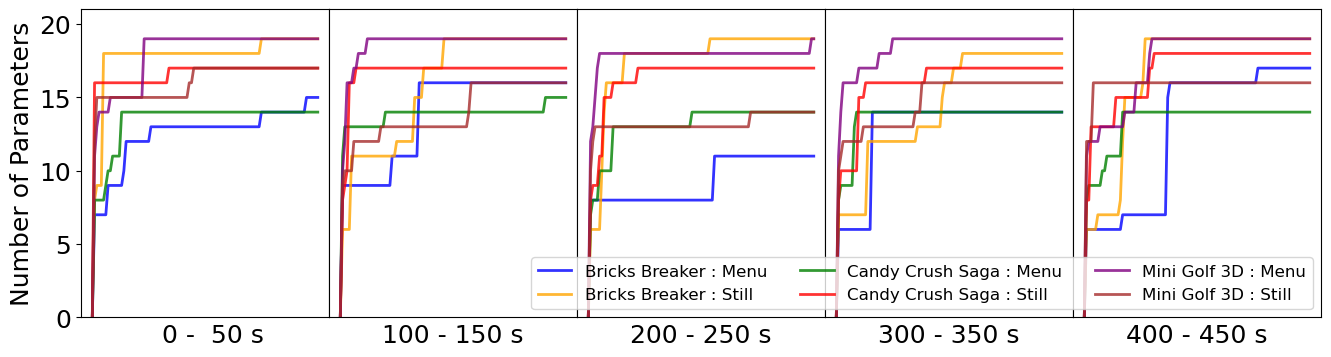
\includegraphics[width=\textwidth]{figures/004_Pixel4_cummulative_parameters.png}
    \vspace{-0.1in}
    \caption{The cumulative number of unique parameters over app run duration in five 50-second segments on Pixel 4. Fixing the x axis.}
    \label{fig:number_parameters_vs_duration_100s}
    \vspace{-0.1in}
\end{figure*}

\paragraph{How Many Systems of Equations?}
\label{subsec:relation}
Since our app run duration  are of 250 seconds each, under macro-scale SPMD  considering an interval $t_e$  between 1s to 5s, 
we can have between 100 to 250 equations.
To explore how many equations should be used,
we first measure how the number of unique model parameters varies with of the app run duration . 

Figure~\ref{fig:number_parameters_vs_duration} shows 
the cumulative number of unique power model parameters for Pixel 4 over a 250-second app run duration
for the six app scenarios . We make the following observations.
(1) The number of unique model parameters increases with the app run duration, reaching a maximum of 15 (for the Candy Crush Saga Menu scenario) to 19 for (the Mini Golf 3D Menu scenario). 
%over 500 seconds for the six app scenarios. 
(2) While the GPU stayed at one frequency and contributed 2 parameters (Busy and Idle power in that frequency) for all the 6 app scenarios,the remaining 13 to 17 are CPU core model parameters.
Similar trends are also observed for the other two  phones.

Figure~\ref{fig:number_parameters_vs_duration} does not show 
the number of unique model parameters in the smaller segments of the app run.
To see this, we plot in Figure~\ref{fig:number_parameters_vs_duration_100s} the 
cumulative number of unique model parameters over  each of 50 seconds time segment , 
for the 6 app scenarios.
We see that the curves for all of the 5 ,50-second segments look very similar, 
suggesting the apps' usage of both the CPU and GPU are similar. 
However, the total number of unique model parameters in each of the 50-second segment
may be lower when compared with the 250-second interval.
For example,on Pixel 4 with Bricks Breaker Menu  the number of parameters
for 0-250s interval is 18 and whereas for the 5 smaller segments number of parameters reduces to 15, 16, 11, 14 and 17.
This suggests that creating a system of equations for the smaller intervals 
may have fewer unknowns depending on the app scenarios.

\cut{ 
\begin{figure}[tp]
    \centering
    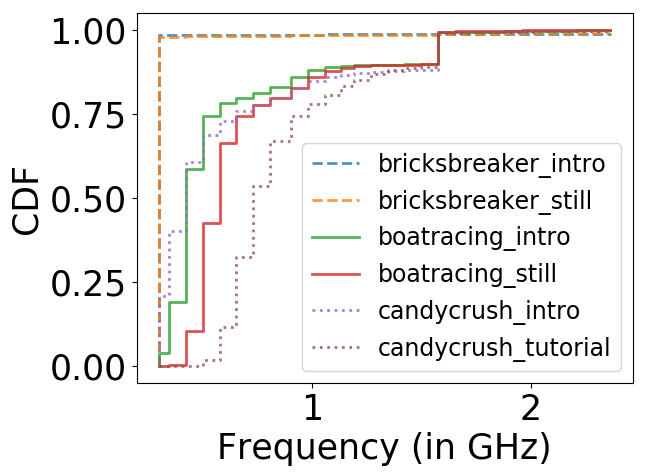
\includegraphics[width=0.65\columnwidth]{figures/cdf_frequency_residence.png}
    \vspace{-0.1in}
    \caption{CDF of the total time spent in each CPU frequencies for 6 app scenarios.}
    \label{fig:cdf_frequency_residence}
    \vspace{-0.1in}
\end{figure}

Finally, to understand how the utilization of different model parameters vary,
we plot in Figure~\ref{fig:cdf_frequency_residence} 
the CDF of the percentage of the total time (250 seconds) spent in each CPU core frequency for the six scenarios. We see the utilizations are uneven: the top 5 parameters in each app scenario
account for 75.20\% to 98.76\% of the total app run duration across the 6 app scenarios.
In contrast, the utilization of the single GPU frequency experience in each app scenario 
varies between 14.72\% and 64.51\%.
}

\begin{figure*}[tp]
    \centering
     \begin{subfigure}[b]{0.32\textwidth}
         \centering
         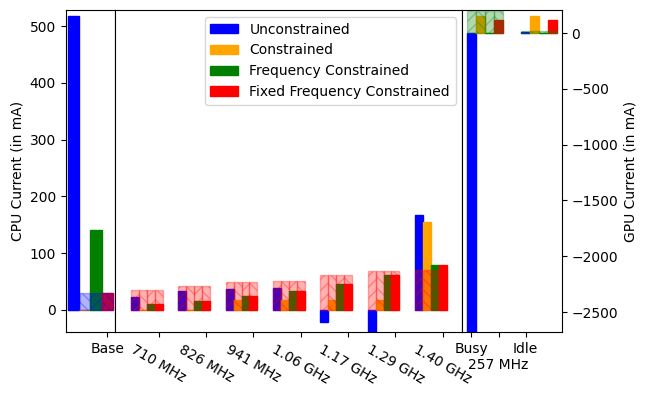
\includegraphics[width=\textwidth]{figures/004_Pixel4_bricksbreaker_menu_50_1_equations.png}
         % \caption{500 equations with 1 second equation interval}
         \label{fig:number_parameters_vs_duration_100s_0}
     \end{subfigure}
    \begin{subfigure}[b]{0.32\textwidth}
         \centering
         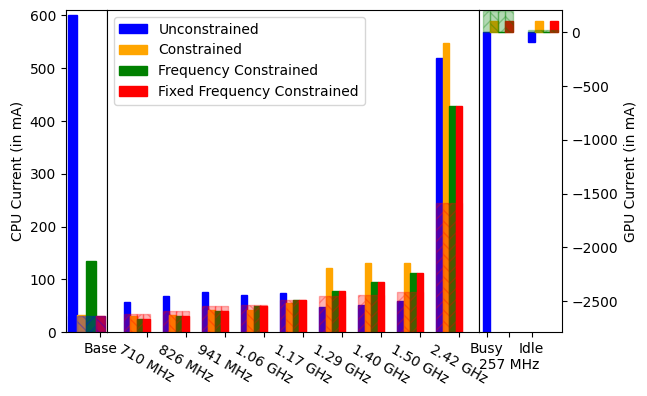
\includegraphics[width=\textwidth]{figures/004_Pixel4_bricksbreaker_menu_250_1_equations.png}
         % \caption{250 equations with 2 seconds equation interval}
         \label{fig:number_parameters_vs_duration_100s_100}
     \end{subfigure}
    \begin{subfigure}[b]{0.32\textwidth}
         \centering
         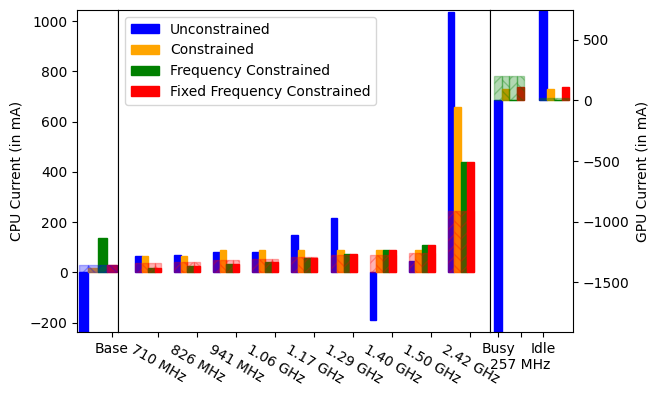
\includegraphics[width=\textwidth]{figures/004_Pixel4_bricksbreaker_menu_250_5_equations.png}
         % \caption{100 equations with 5 seconds equation interval}
         \label{fig:number_parameters_vs_duration_100s_200}
     \end{subfigure}
     \hfill
         \centering
     \begin{subfigure}[b]{0.32\textwidth}
        \centering
    	{ \scriptsize
    	\begin{tabular}{ | l | c | c | c | c | c | c | }
    		\hline
    		     & \multicolumn{6}{ c|}{Error for each App Scenarios (in \%)}\\
    		\cline{2-7}
                    Model & \rot{B. Menu} & \rot{B. Still} & \rot{C. Menu} & \rot{C. Still} & \rot{M. Menu} & \rot{M. Still}  \\
    		\hline
                Unconst.             & 0.7 & 0.9 & 0.8 & 1.1 & 1.0 & 0.9 \\
                Const.               & 1.2 & 1.1 & 1.2 & 1.6 & 1.4 & 1.3 \\
                Freq. Const.         & 1.2 & 1.1 & 1.6 & 2.1 & 1.9 & 1.8 \\
                Fix. F. Const.       & 1.2 & 1.1 & 1.6 & 2.1 & 1.9 & 1.8 \\
                Classical            & 37 & 45 & 17 & 24 & 27 & 9.2 \\
    		\hline
    	\end{tabular}
    	}
	\caption{50 equations with 1 second equation interval}
    \end{subfigure}
     \begin{subfigure}[b]{0.32\textwidth}
        \centering
    	{ \scriptsize
    	\begin{tabular}{ | l | c | c | c | c | c | c | }
    		\hline
    		     & \multicolumn{6}{ c|}{Error for each App Scenarios (in \%)}\\
    		\cline{2-7}
                    Model & \rot{B. Menu} & \rot{B. Still} & \rot{C. Menu} & \rot{C. Still} & \rot{M. Menu} & \rot{M. Still}  \\
    		\hline
                Unconst.             & 0.8 & 0.7 & 1.4 & 1.4 & 1.1 & 1.2 \\
                Const.               & 1.0 & 0.8 & 1.3 & 1.5 & 1.2 & 1.3 \\
                Freq. Const.         & 1.0 & 0.9 & 1.4 & 1.8 & 1.3 & 1.4 \\
                Fix. F. Const.       & 1.0 & 0.9 & 1.4 & 1.8 & 1.3 & 1.4 \\
                Classical            & 37 & 45 & 17 & 24 & 27 & 8.5 \\
    		\hline
    	\end{tabular}
    	}
	\caption{250 equations with 1 second equation interval}
    \end{subfigure}
         \begin{subfigure}[b]{0.32\textwidth}
        \centering
    	{ \scriptsize
    	\begin{tabular}{ | l | c | c | c | c | c | c | }
    		\hline
    		     & \multicolumn{6}{ c|}{Error for each App Scenarios (in \%)}\\
    		\cline{2-7}
                    Model & \rot{B. Menu} & \rot{B. Still} & \rot{C. Menu} & \rot{C. Still} & \rot{M. Menu} & \rot{M. Still}  \\
    		\hline
                Unconst.             & 0.4 & 0.4 & 0.7 & 0.7 & 0.5 & 0.6 \\
                Const.               & 0.6 & 0.4 & 0.8 & 0.9 & 0.6 & 0.8 \\
                Freq. Const.         & 0.7 & 0.5 & 1.0 & 1.2 & 0.9 & 1.1 \\
                Fix. F. Const.       & 0.7 & 0.5 & 1.0 & 1.2 & 0.9 & 1.1 \\
                Classical            & 37 & 45 & 17 & 24 & 27 & 8.5 \\
    		\hline
    	\end{tabular}
    	}
	\caption{50 equations with 5 second equation interval}
    \end{subfigure}
    \caption{3 ways of creating the system of equations for Bricks Breaker Menu scenario on Pixel 4. (Only model parameters for 9 CPU frequencies with highest utilization are shown due to space constraint.). Showing error for all app scenarios. \comment{Fixing the negative part of the plots.}}
    \label{fig:macro_3_ways}
    \vspace{-0.1in}
\end{figure*}

Based on the above exploration, we experimented with 3 alternatives for creating the system of equations for each app scenario, by varying
the app run duration per system between 100, and 250 seconds, and
the interval  per equation between 1, and 5 seconds, while ensuring that the number
of equations per system is 50 or more.

The solutions found with  these  3 alternatives of creating systems of equations for Bricks Breaker Menu scenario on Pixel 4 are
shown in the Figure~\ref{fig:macro_3_ways}. For comparison, we present the model parameters 
derived from traditional power model derivation by hatched bars. Note that for GPU parameters 
shown for the TPMD models is derived for the specific app scenario using Figure 1. In general, models derived using TPMD are app-agnostic. Due to page limit, we omit including all the results
found for the remaining app scenarios and 
on other phones , however the findings are very similar.
% First, we observe that the ranks of the systems are more than 1 less than the number of model parameters
% when the equation covers 100 or 200 seconds, and are 1 less than the number of parameters for 500-second app duration. The reason for this is that the base power shows up in all equations which does not contribute to the rank.
First, we observed that the ranks of the system of equations  is less than the number of model parameters by more than 1. 
The reason for this is that the base power shows up in all equations which does not contribute to the 
rank. 

As expected, since the systems are under-ranked,
the model parameters output from the regression solver look very different from those found from the classic model. 
For the {\it unconstrained solver},
the parameters generated, shown in Figure~\ref{fig:macro_3_ways},
violate some basic properties:
(1) some model parameters generated are negative, \eg the the CPU component power at 1.49 GHz is -69.70 mA for 100 intervals x 1sec  and 1.62 GHz is -3116.8 mA for 50 intervals x 5sec systems, and 
(2) the CPU power draw at a lower frequency is often higher than the power draw at a higher frequency (for all the 3 systems), and 
(3) the GPU Idle power draw generated is higher than the GPU Busy power (for all the 3 systems).

For the {\it constrained solver}, while the parameters generated, shown as 
"Constrained" in Figure~\ref{fig:macro_3_ways}, are all
positive and no more non-decreasing with increasing frequencies, the CPU power parameters
still do not satisfy the monotonicity property; the parameters for consecutive frequencies
often stay the same. For example, for the Bricks Breaker Intro scenario, 
the CPU power stays at 42.02 mA for 4 of the frequencies from 710 MHz to 1.05 GHz and again remains at 75.35 mA for 5 of the frequencies from 1.29 GHz to 1.61 GHz for the 50x5 system.

For Frequency-constrained solver,  the parameters generated, shown in in Figure~\ref{fig:macro_3_ways}, look very much similar to those in the classic model, but 
the base power draw ranges between 101.1 mA to 108.3 mA, 
which is over 3.3 times higher than their counterpart of 30.12 mA observed in the classic model.

% 41.36 mA, 33.98 mA and 30.12 mA for Pixel 2, Moto Z3 and Pixel 4
To overcome the under-rank problem, we fixed the base power to  the  constant value of 30.12 mA as in case of classic model which makes the rank equal to the  number of parameters for 
the two systems with 250-second duration, 250x1 and 50x5.  
% in the rows labeled "Fix-Freq-Constr.",
With this approach ,the parameters generated by the solver,only changed slightly; the solver splited the excessive base power and shifted it into the GPU 
Busy and Idle power and the trend of all the parameters now look similar to those observed in the classic model. 
% 
% \comment{However, the specific model parameters (excluding the base power) 
% differ from those in the classic model in two major ways.
% % (1) the individual CPU power parameter values in the two systems
% % 500x1 and 100x5 are between 0\% and 21.35\% lower than
% % their counterparts in the classic model.
% (1) the individual CPU power parameter values in the two systems are 
% 11.27\% to 96.96\% lower for 500x1 and 11.84\% to 96.78\% lower for 100x5 than
% their counterparts in the classic model.
% (2) The GPU Busy and Idle powers are identical, when the GPU Idle power is supposed to be 4$\times$ lower than the GPU Busy power.  
% }


\if 0
We make the following observations.
(1) The CPU power parameter now increases with the frequency similarly as in the classical model
and achieves between 0.55\% and 3.46\% Least Square Fitting error, 
which are lower than the error of between 5.78\% and 10.74\% archived by 
the classic model, for the four app scenarios. 
(3) However, the specific parameter values at individual frequencies differ significantly from their counterparts in the classical model. For example, 
the CPU power for 1.65 GHz is 76.23 mA in the classical model
but 28.84 mA and 44.19 mA by SPMD for the Boat Racing Intro and Candy Crush Saga Intro scenarios, respectively. Similarly, the base power ranges between 88.73 mA to 242.3 mA for the four scenarios
but is only 27.86 mA in the classic model. 
Further, the GPU power parameters are significantly underestimated: the Busy parameter under 342 MHz
ranges between 0 mA and 168.8 mA  for the two scenarios of Boat Racing but are 253.7 mA and 358.0 mA in the classic model, respectively.
\fi
% \questionaj{This is because of unconstrained GPU. Does physics inform us about any constraints for GPU other than just monotonicity.}

\paragraph{Parameters for all app scenarios.}
Using the 250x1 system of equations, we applied the Fix-Freq-Constr. version of SPMD 
to all the 6 app scenarios. Figure~\ref{fig:macro_freq_constr} shows that the model parameters generated with Fix-Freq-Constr 
suffer simillar two problems as observed in the case of the Boat Racing Intro scenario.

\begin{figure*}[tp]
    \centering
     \begin{subfigure}[b]{0.32\textwidth}
         \centering
         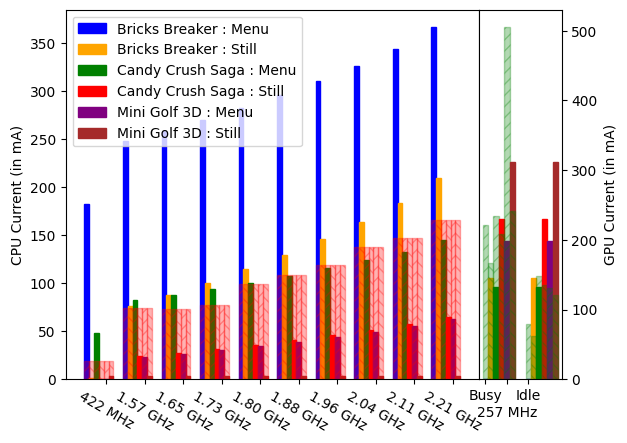
\includegraphics[width=\textwidth]{figures/002_Pixel2_250_5_macro_equations.png}
         \label{fig:number_parameters_vs_duration_100s_0}
     \end{subfigure}
    \begin{subfigure}[b]{0.32\textwidth}
         \centering
         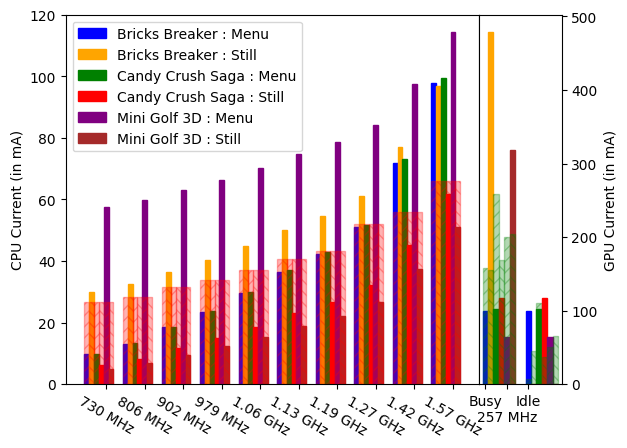
\includegraphics[width=\textwidth]{figures/003_MotoZ3_250_5_macro_equations.png}
         \label{fig:number_parameters_vs_duration_100s_100}
     \end{subfigure}
    \begin{subfigure}[b]{0.32\textwidth}
         \centering
         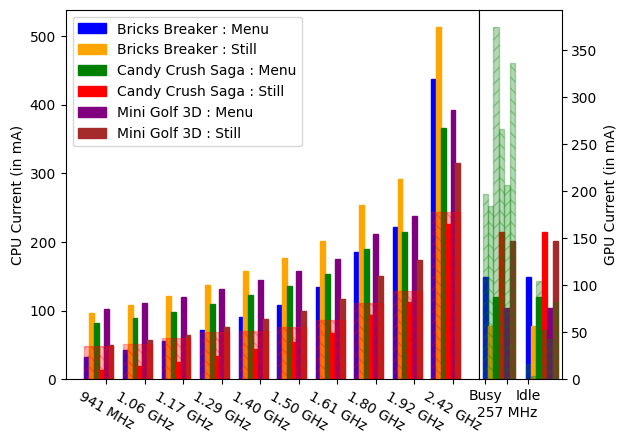
\includegraphics[width=\textwidth]{figures/004_Pixel4_250_5_macro_equations.png}
         \label{fig:number_parameters_vs_duration_100s_200}
     \end{subfigure}
     \hfill
     \centering
     \begin{subfigure}[b]{0.32\textwidth}
        \centering
    	{ \scriptsize
    	\begin{tabular}{ | l | c | c | c | c | c | c | }
    		\hline
    		     & \multicolumn{6}{ c|}{Error for each App Scenarios (in \%)}\\
    		\cline{2-7}
                    Model & \rot{B. Menu} & \rot{B. Still} & \rot{C. Menu} & \rot{C. Still} & \rot{M. Menu} & \rot{M. Still}  \\
    		\hline
                Fix. F. Const.       & 0.9 & 1.1 & 1.2 & 0.6 & 0.8 & 0.7 \\
                Classical            & 18 & 28 & 13 & 3.4 & 45 & 6.0 \\
    		\hline
    	\end{tabular}
    	}
	\caption{Pixel 2}
    \end{subfigure}
         \begin{subfigure}[b]{0.32\textwidth}
        \centering
    	{ \scriptsize
    	\begin{tabular}{ | l | c | c | c | c | c | c | }
    		\hline
    		     & \multicolumn{6}{ c|}{Error for each App Scenarios (in \%)}\\
    		\cline{2-7}
                    Model & \rot{B. Menu} & \rot{B. Still} & \rot{C. Menu} & \rot{C. Still} & \rot{M. Menu} & \rot{M. Still}  \\
    		\hline
                Fix. F. Const.       & 1.8 & 0.3 & 2.6 & 0.4 & 0.2 & 26 \\
                Classical            & 39 & 11 & 31 & 19 & 5.9 & 39 \\
    		\hline
    	\end{tabular}
    	}
	\caption{Moto Z3}
    \end{subfigure}
         \begin{subfigure}[b]{0.32\textwidth}
        \centering
    	{ \scriptsize
    	\begin{tabular}{ | l | c | c | c | c | c | c | }
    		\hline
    		     & \multicolumn{6}{ c|}{Error for each App Scenarios (in \%)}\\
    		\cline{2-7}
                    Model & \rot{B. Menu} & \rot{B. Still} & \rot{C. Menu} & \rot{C. Still} & \rot{M. Menu} & \rot{M. Still}  \\
    		\hline
                Fix. F. Const.       & 0.7 & 0.5 & 1.0 & 1.2 & 0.9 & 1.1 \\
                Classical            & 37 & 45 & 17 & 24 & 27 & 8.5 \\
    		\hline
    	\end{tabular}
    	}
	\caption{Pixel 4}
    \end{subfigure}
     \hfill
    \caption{Model parameters derived by macro-scale SPMD for 50x5 system on the 3 phones. The classic models for GPU are from Figure~\ref{fig:gpu_model}. (Only model parameters for 10 CPU frequencies with highest utilization are shown due to space constraint.) Hatched bars represents the classical model coefficients.}
    \label{fig:macro_freq_constr}
    \vspace{-0.1in}
\end{figure*}

\subsection{Analysis}
We dig deeper into one of the the full-rank system, \ie 50x5, to understand why 
SPMD generates very different parameters compared to the classic model. 
\comment{
Since the rank of the system is already full, we calculated the singular values for these equations.
Table~\ref{tab:macro_singularvalues} shows that each of the system of equations has only 1 dominating singular value, 
suggesting that the matrix (formed by coefficients of unknown variables in the left-hand-side of those equations) has only one dominating direction. This indicates that all the equations are basically describing the same state of power usage, and thus lack diversity.
}
% These results suggest the equations lack diversity in terms of component usage. 

\begin{table*}[tp]
% \questionaj{Also add rank of freq-constrained case}
{\small
    \centering
    \caption{The rank and singular values for the set of equations for macro-scale "Fix-Freq.-Constr. SPMD" for 50x5 system on Pixel 4. (Top 11 singular values are shown.)}
    \vspace{-0.1in}
    \begin{tabular}{|c|c|c|c|c|c|c|c|c|c|c|c|c|c|c|c|}
    \hline
        App & Scenario & \# of Eqns. & \# of Vars. & Rank &  \multicolumn{11}{c|}{Singular Values} \\
        \hline
         \multirow{2}{15mm}{Bricks Breaker} & Menu & 50 & 18 & 17 & 6.54  & 0.37  & 0.17  & 0.10  & 0.04  & 0.02  & 0.02  & 0.01  & 0.01  & 0.00  & 0.00 \\
         \cline{2-16}
         & Still &  50 & 19 & 16 & 6.73  & 0.38  & 0.34  & 0.16  & 0.03  & 0.02  & 0.02  & 0.01  & 0.01  & 0.01  & 0.00 \\
         \hline
        \multirow{2}{15mm}{Candy Crush Saga} & Menu &  50 & 19 & 19 & 6.79  & 0.49  & 0.19  & 0.10  & 0.08  & 0.03  & 0.03  & 0.02  & 0.02  & 0.01  & 0.01 \\
         \cline{2-16}
         & Still & 50 & 17 & 17 & 6.81  & 0.52  & 0.21  & 0.10  & 0.05  & 0.05  & 0.03  & 0.02  & 0.01  & 0.01  & 0.01 \\
         \hline
        \multirow{2}{15mm}{Mini Golf 3D} & Menu & 50 & 19 & 19 & 6.41  & 1.62  & 0.47  & 0.38  & 0.18  & 0.06  & 0.03  & 0.02  & 0.02  & 0.01  & 0.01 \\
        \cline{2-16}
	     & Still & 50 & 17 & 17 & 6.46  & 0.99  & 0.34  & 0.19  & 0.11  & 0.06  & 0.04  & 0.03  & 0.02  & 0.01  & 0.01 \\
	     \hline
    \end{tabular}
    \label{tab:macro_singularvalues}
    \vspace{-0.1in}
}
\end{table*}

% \questionaj{I don't think next 2 paragraphs are necessary. Low rank 
% already established  that the model equations have little diversity}
% In addition to the low ranks of the systems of model equations under the macro-scale,
% suggesting the equations lack diversity in terms of component usage, 

In addition to lack of diversity in phone component usage which contributed 
to the sparse singular values, we found that the energy values in LHS of the equation   appear to contain 
measurement noise which further prevents the regression solver from generating meaningful solutions.
To see this, we plot the distribution of the LHS energy values of the 
equations in the two systems 250x1 and 50x5, 
% \ie the energy values for the 50 1-second intervals.
Figures~\ref{fig:y_distribution}(a)-(b) 
show the energy values for the two systems are clustered in a Gaussian distribution with standard deviation of 3.04 mA and 5.72 mA, 
each of which is less than 2.45\% compared with the mean value.
This Gaussian-like distribution suggests that the LHS values of the equations contain
measurement noise.
\comment{this is not obvious????}

\begin{figure}[tp]
    \centering
         \begin{subfigure}[b]{0.49\columnwidth}
         \centering
         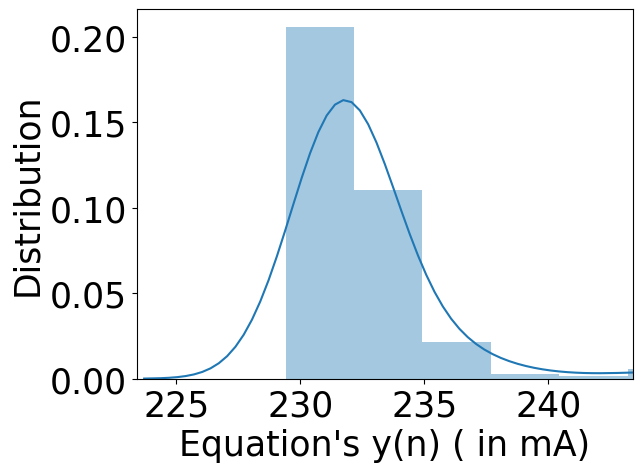
\includegraphics[width=\textwidth]{figures/004_Pixel4_bricksbreaker_menu_250_1_distribution_y_n.png}
         \caption{250 1-second equations.}
         \label{fig:y_n_boatracing_intro_1_500}
    \end{subfigure}
    \hfill
    \begin{subfigure}[b]{0.49\columnwidth}
         \centering
         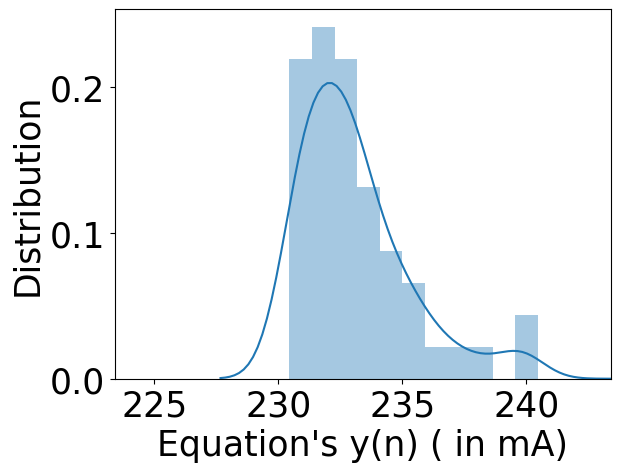
\includegraphics[width=\textwidth]{figures/004_Pixel4_bricksbreaker_menu_250_5_distribution_y_n.png}
         \caption{50 5-second equations.}
         \label{fig:y_n_boatracing_intro_5_500}
    \end{subfigure}
    \caption{Distribution of the energy terms of the
    equations for Bricks Breaker Menu scenarios on Pixel 4.}
    \label{fig:y_distribution}
\end{figure}

\if 0
Mathematically, since the small variations of the equations
all fall in a small volume of the multidimensional space, 
multiple solutions, from different constraints, 
that all have similar error, become possible as shown in Figure~\ref{fig:mutiple_equations}.

\begin{figure}[tp]
    \centering
    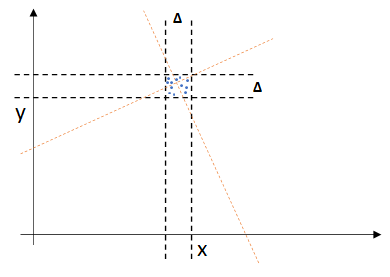
\includegraphics[width=0.70\columnwidth]{figures/mutiple_equations.png}
    \vspace{-0.1in}
    \caption{Multiple solutions (from different constraints) give similar errors due to low equation diversity.}
    \label{fig:mutiple_equations}
    \vspace{-0.1in}
\end{figure}
\fi



\if 0
\begin{figure}[hp]
    \centering
    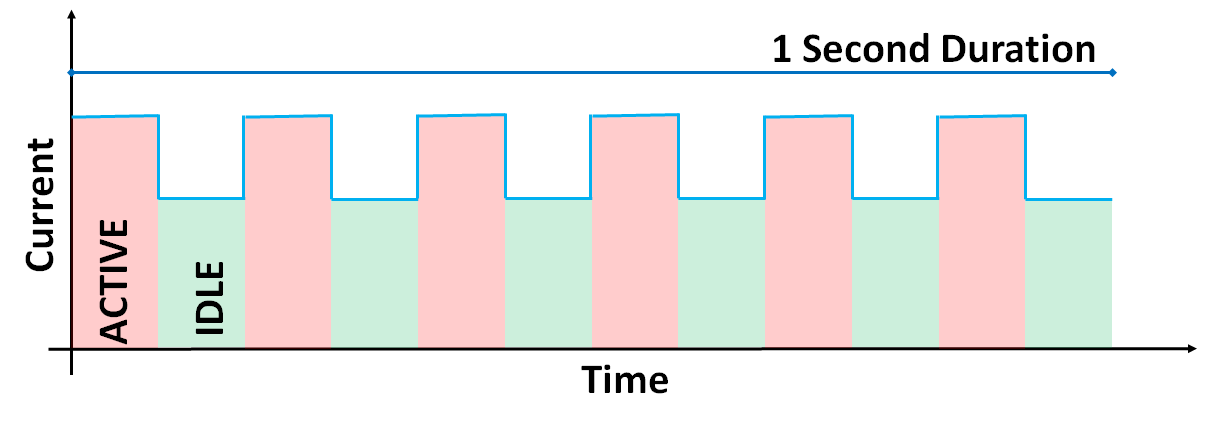
\includegraphics[width=0.95\columnwidth]{figures/coarse_grained_2.png}
    \vspace{-0.1in}
    \caption{The equations are too coarse grained}
    \label{fig:coarse_grained}
    \vspace{-0.1in}
\end{figure}
\fi

\begin{figure}[tp]
    \centering
    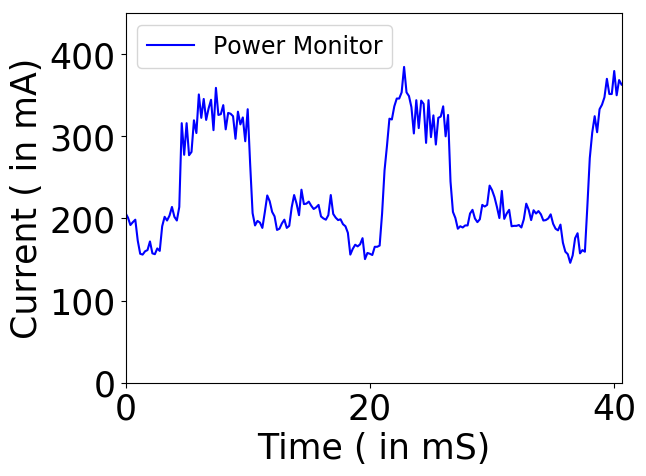
\includegraphics[width=0.50\columnwidth]{figures/candy_crush_saga_tutorial_timeline.png}
    \vspace{-0.1in}
    \caption{A snippet of power monitor readings for Candy Crush Saga Menu scenario on Moto Z3.}
    \label{fig:power_trace_candycrushturorial}
    \vspace{-0.1in}
\end{figure}

To understand why the system of model equations for the 6 app scenarios lack diversity, 
we zoom into the power monitor readings. Figure~\ref{fig:power_trace_candycrushturorial}
shows a snippet of the power monitor readings during the Candy Crush Saga Tutorial scenario. 
We see that the power draw shows a clear repeating pattern every 16.7ms duration.
This happens due to typical game app behavior -- a game app typically
renders 60 FPS and the graphic contents rendered within each game scenario are largely similar.
As a result, aggregating the power activities within each of the one-second interval into one model equation
will result in the (set of ??) equations (for the same app scenario) looking largely similar. 

% The smartphones run at a given frames per second (with an upper limit). For Moto Z3 at max 60 frames can be displayed on the screen. Frames per second is dictated by the application running. The game apps generate frames at 60 FPS which translates to 1 frame getting rendered and displayed every 16.7 ms.
%% 6b. Explain that variation is in 16.7mS

To summarize,our experiments and analysis above suggest
that the equations created from macro-scale SPMD do not exhibit enough diversity 
and as a result the regression solver can not output meaningful solutions for the model parameters.

% to conclude that we need to dig deeper and to have much smaller equation duration for retaining state change information needed to solve the set of equations meeting our goals explained in~\S\ref{sol:goals}.